\documentclass{DateStructure}

\SubjectName{算术表达式求值演示}
\CollegeName{理学院}
\Major{信息与计算科学}
\GroupNumber{第十六组}
\StudentA{20071226}{童繁}{进程图}
\StudentB{20071227}{王瀚功}{测试}
\StudentC{20071228}{王赛豪}{文案}
\StudentD{20071229}{吴政豪}{调试}
\StudentE{20071230}{武琦}{代码}

\begin{document}	
\makecover
\newpage
\thispagestyle{empty}
\tableofcontents   

\newpage
\setcounter{page}{1}  
	
\section{需求分析}
\begin{itemize}
\item[(1)]设计一个程序,以字符序列的形式从终端输入语法正确的、不含变量的整数表达式,演示用算符优先法对算术四则混合运算表达式的求值;
\item[(2)]演示在求值中运算符栈、运算数栈、输入字符和主要操作的变换过程;
\item[(3)]扩充运算符集,如增加乘方、开方等运算;
\item[(4)]运算量可以是变量;
\item[(5)]计算器的功能和仿真界面。
\end{itemize}

\section{项目亮点}
\begin{itemize}
\item[(1)]通过Python调用C语言功能函数,实现了仿windows的简易版计算器;
\item[(2)]建立了独立的工作栈库和计算功能库,使得项目的调用更加清晰合理;
\item[(3)]运用txt文本记录求值过程中的操作变换过程,让使用者方便单独使用计算器和查看具体过程;
\item[(4)]解决了在实数范围内的运算;
\item[(5)]区分了除0无意义和输入错误两种情况;
\item[(6)]输入过程可以添加空格;
\item[(7)]运算量可以是已赋值的变量,程序会给出精确结果;
\item[(8)]增加了乘方、开方运算。
\end{itemize}

\section{概要设计}
表达式求值是程序设计语言编译的一个最基本问题,其中任何一个表达式都是由操作数、运算符、界限符组成。要实现算术表达式的演示,需要建立栈的顺序结构来实现栈的基本操作,并构建两个工作栈:一个寄存运算符,另一个寄存操作数和运算结果。在读取时,输出具体的进出栈过程和操作过程。\par
\begin{figure}[H] 
\centering
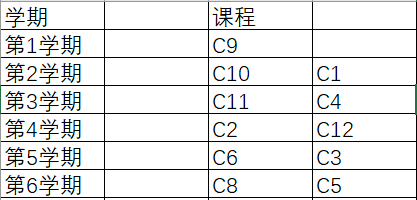
\includegraphics[width=500pt]{1.png}
\caption{结构体系图}
\end{figure}

\section{详细设计}
\subsection{工作栈库}
\begin{figure}[H] 
\centering
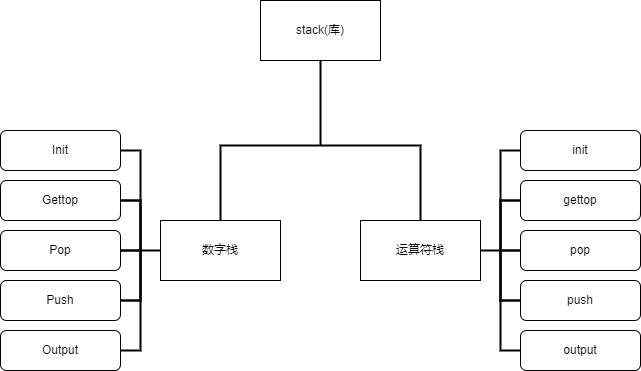
\includegraphics[width=400pt]{stack.png}
\caption{栈库示意图}
\end{figure}
\lstinputlisting[language=C]{./code/stack.h}
\subsection{计算功能库}
\subsubsection{function.h}
\lstinputlisting[language=C]{./code/function.h}
\subsubsection{function.c}
\begin{figure}[H] 
\centering
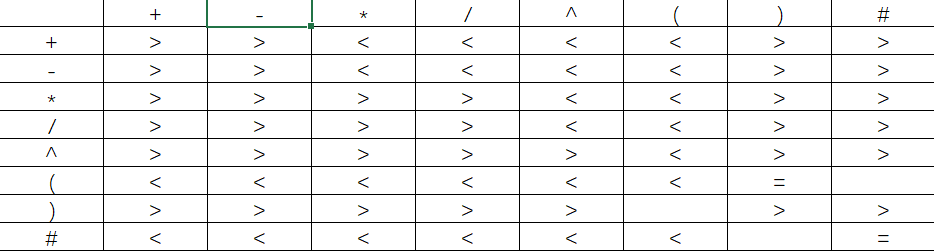
\includegraphics[width=400pt]{2.png}
\caption{算符优先级}
\end{figure}
\begin{figure}[H] 
\centering
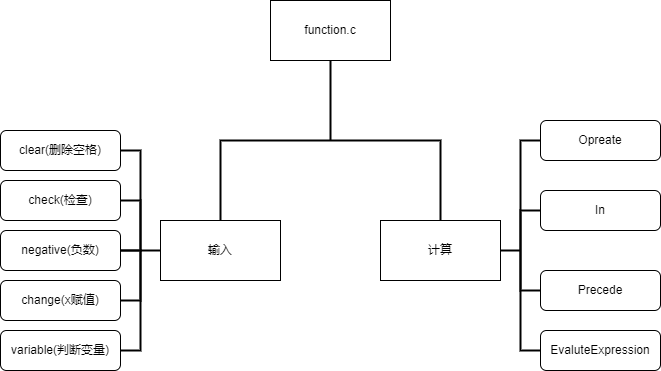
\includegraphics[width=400pt]{function.png}
\caption{计算功能示意图}
\end{figure}
\lstinputlisting[language=C]{./code/function.c}	
\subsection{C的主函数}
\begin{figure}[H] 
\centering
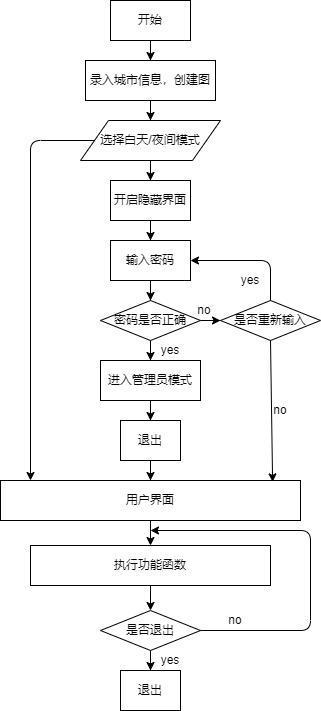
\includegraphics[width=300pt]{主函数.png}
\caption{主函数流程图}
\end{figure}
\lstinputlisting[language=C]{./code/main.c}
\subsection{Python的计算器可视化}
\lstinputlisting[language=Python]{./code/calculator.py}

\section{用户手册}
\subsection{测试数据}
\begin{figure}[H] 
\centering
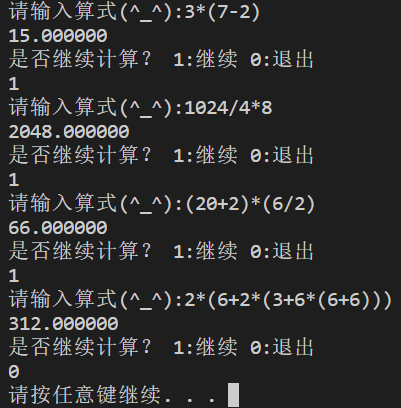
\includegraphics[width=400pt]{测试数据.png}
\caption{测试数据}
\end{figure}
具体过程如下:\par
\subsubsection{3*(7-2)}
\lstinputlisting{测试1.txt}
\subsubsection{1024/4*8}
\lstinputlisting{测试2.txt}
\subsubsection{(20+2)*(6/2)}
\lstinputlisting{测试3.txt}
\subsubsection{2*(6+2*(3+6*(6+6)))}
\lstinputlisting{测试4.txt}
\subsection{功能测试}
\begin{figure}[H] 
\centering
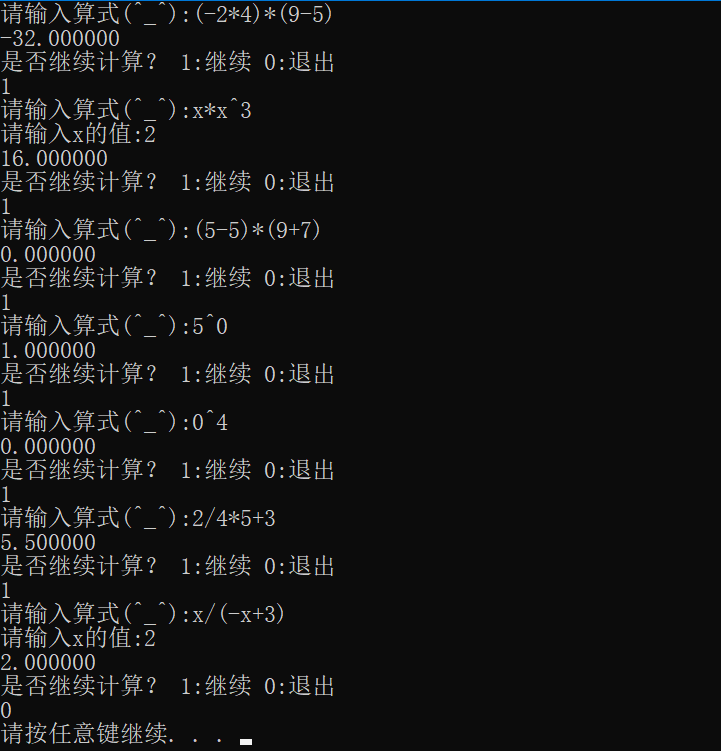
\includegraphics[width=400pt]{功能.png}
\caption{功能测试}
\end{figure}
\subsection{错误案例}
\begin{figure}[H] 
\centering
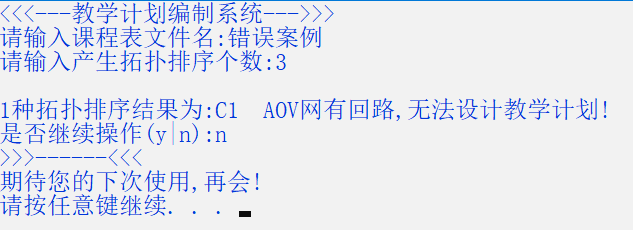
\includegraphics[width=400pt]{错误.png}
\caption{错误案例}
\end{figure}
\subsection{计算器测试}
\begin{figure}[H] 
\centering
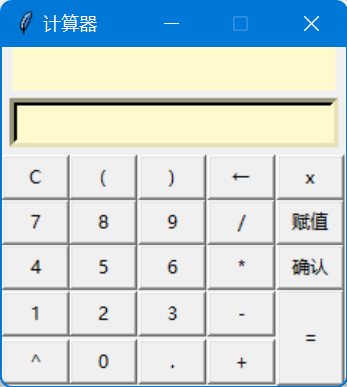
\includegraphics[width=400pt]{计算器.png}
\caption{计算器}
\end{figure}
\begin{figure}[H] 
\centering
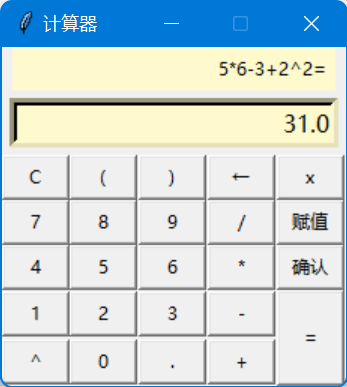
\includegraphics[width=400pt]{计算器2.png}
\caption{输入案例}
\end{figure}
\begin{figure}[H] 
\centering
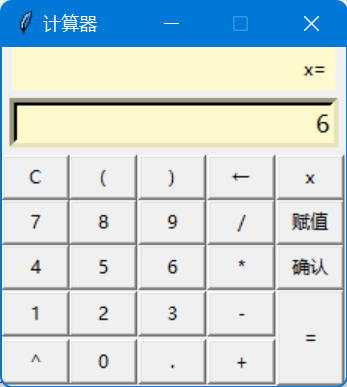
\includegraphics[width=400pt]{赋值.png}
\caption{变量赋值}
\end{figure}

\section{心得体会}
这次课程设计的心得体会通过实践我们的收获如下:\par
1.在这次的计算器算法及界面实现的过程中,我们更深刻的了解栈的特点与用法。\par
2.在不断的修改程序bug的过程中,我们对程序运行的细节更加明了,提高了我们的查错,纠错能力。\par
3.在面对含有变量的算式问题,我们发现可以使用之前课程设计的一元稀疏多项式运算程序来进行设计。\par
4.在界面设计中我们学习了DLL库的设计,将设计的C语言程序加载到Python程序中,实现计算器界面。\par

\newpage 
\section{附录}
\subsection{stack.h}
\lstinputlisting[language=C]{./code/stack.h}
\subsection{stack.c}
\lstinputlisting[language=C]{./code/stack.c}
\subsection{function.h}
\lstinputlisting[language=C]{./code/function.h}
\subsection{function.c}
\lstinputlisting[language=C]{./code/function.c}
\subsection{main.c}
\lstinputlisting[language=C]{./code/main.c}
\subsection{calculator.py}
\lstinputlisting[language=Python]{./code/calculator.py}
\end{document}
